\documentclass{article}
\usepackage[utf8]{inputenc}
\usepackage{braket}
\usepackage{amsmath}
\setlength{\parskip}{\baselineskip}%
\setlength{\parindent}{0pt}%
\usepackage{graphicx}


\title{Deep learning Homework 1}
\author{tylertracy1999 }

\begin{document}

\maketitle


\section*{Question 1, Derivatives}

a) What is Jacobian matrix? $J_y^{(k)}(z^{(k)})$?

The Jacobian matrix is the matrix of all the derivatives of the inputs with respect to the output. It will be of dimensions $D \textbf{x} M$

$$\begin{bmatrix}
	\frac{\partial y_1}{\partial z_1} & \dots & \frac{\partial y_1}{\partial z_D} \\
	\vdots & \ddots & \\
	\frac{\partial y_M}{\partial z_1} & \dots & \frac{\partial y_M}{\partial z_D} \\
\end{bmatrix}$$

b) If function f is a scalar function as follows, what is Jacobian matrix $J_y^{(k)}(z^{(k)})$

When this is true, this means that instead of $y = f(z)$, we have $y_i = f(z_i)$. Meaning that each value of y solely depends on the corresponding value of z. Since we have this 1-1 relationship, the Jacobian matrix is now square. Also The diagonals of the Jacobian are 0 since values of z only change when their since corresponding value of y changes.


$$\begin{bmatrix}
	\frac{\partial y_1}{\partial z_1} & 0 & \dots & 0 \\
	0 & \frac{\partial y_2}{\partial z_2} & \dots & 0 \\
	\vdots & \vdots & \ddots & 0 \\
	0 & \dots & 0 & \frac{\partial y_M}{\partial z_D} \\
\end{bmatrix}$$

\section*{Question 2, Multivariate Quadratic}


$ E = \frac{1}{2} w^TAw + w^Tb+c$

Parameters are updated: $w^{(k+1)} = w^{(k)} - \eta \nabla_w E$


What is the optimal learning rate?

Since A is diagonal, that means that all of the $w_i$'s are decoupled. That means this is a sum of $N$ quadratic functions.

$$ E = \frac{1}{2}\sum_{i}(a_{ii}w_i^2 + b_iw_i + c) $$

Our goal is to get w to update to the minimum of the function. Since these are all quadratics, we can find the minimum by taking the derivative and setting it equal to 0. We can then solve for w.

Lets find the optimal learning rate for a single quadratic. The update rule for a single quadratic is:

$$ w^{(k+1)} = w^{(k)} - \eta \frac{\partial E}{\partial w} $$

The optimal learning rate means that $w^{(k+1)}$ will be the minimum, i.e. we got to the minimum in one step. So n should be the distance between the current w and the minimum w. We can find the minimum by taking the derivative and setting it equal to 0. We can then solve for w.

$$ E' = a_{ii}w + b_i $$
$$ w_i = -\frac{b_i}{a_{ii}} $$

Now we can plug these values into the update rule and solve for the optimal learning rate.

$$ -\frac{b}{a} = w - \eta (a_{ii}w + b_{i}) $$
$$ \eta(a_{ii}w + b_{i}) = w + \frac{b_i}{a_{ii}} $$
$$ \eta = \frac{wa_{ii} + b_i}{a_{ii}} * \frac{1}{a_{ii}w + b_{i}} $$
$$ \eta = \frac{1}{a_{ii}}$$

So the optimal learning rate for a single quadratic is $\frac{1}{a_{ii}}$. The learning rate has to be the same for all quadratics since it is constant. A learning rate that is over twice the optimal learning rate will diverge so we want to pick a learning rate where $\eta < 2 \eta_{i,opt}$ this will prevent the update rule from diverging in every direction.


\section*{Question 3, Gradient Descent}

What is Gradient Decent? What are the pros and cons of Gradient Decent?

Gradient Decent is a method of finding the minimum of a function. The basic idea is to make a random guess at where the minimum is and then compute the gradient of the function at that point. The negative gradient will point to the direction of steepest descent. If we move in that direction with a constant step and well calculated step size, then the algorithm will eventually converge on the minimum.

The pros of this method is that it is simple and quick for simple functions. It is also easy to implement. It is also normally quicker since it runs through all the training data then makes the update

The cons are it can easily get stuck on saddle points or local minima. It can also be slow for complex functions


What is Stochastic Gradient Decent? What are the pros and cons of Stochastic Gradient Decent?


Stochastic Gradient Decent is different from normal Gradient Decent because instead of moving in the direction of the negative gradient of all of the data points, it moves in the direction of the negative gradient of a single data point.
This mechanisms help to stay away from local minimums, because if you hit a local minimum in one data point's gradient, the next iteration could point you a different way away from that.

The cons of Stochastic Gradient Decent is that it takes longer because it has to update the model after each data point in the training set instead of after the whole training set is done.

What is Mini-Batch Gradient Decent? What are the pros and cons of Mini-Batch Gradient Decent?

Mini-Batch Gradient Decent is a combination of Stochastic Gradient Decent and Gradient Decent. It takes a subset or "batch" of data points and computes the gradient of the batch. It then updates the model in the direction of the negative gradient of the batch.

The pros of this is that it helps to avoid local minima and saddle points, and it is faster than Stochastic Gradient Decent because it doesn't have to update the model after every data point.

The cons of this is that is that you have another hyper parameter to tune which is the mini-batch size



\section*{Question 4, Regularization}

What is each of the following regularization and how does it help deep neural network?

a. (3 points) Batch normalization.

Batch normalization is a way of normalizing the input data such that they have a mean of 0 and a standard deviation of 1. This essentially acts as another layer on the model and it can be applied after every layer. This helps the model by making the data it receives more uniform and thus easier to train and lessens the chance of the model over-fitting.

b. (3 points) Drop out.

In dropout regularization every iteration of training, a random set of neurons are dropped out of the network. This helps the network to generalize better and prevent over-fitting. It also helps to prevent the network from relying on a single neuron.

The number of nodes to drop each iteration is another hyper parameter that needs to be tuned.


c. (3 points) L1/L2 regularization.

L1 and L2 regularizations assume that over-fitting comes from the weights of the model being too large. They both add a penalty to the cost function.

For L1 the regularized cost function looks like:

$$ Cost = Loss + \lambda \sum_{i} |w_i| $$

And for L2 the regularized cost function looks like:

$$ Cost = Loss + \lambda \sum_{i} w_i^2 $$

The $\lambda$ is a new hyper parameter that we have to tune. The larger the $\lambda$ the more the weights will be penalized.

These help the model by preventing over-fitting. They do this by preventing the weights from getting too large which is a good indicator of overfitting.

d. (3 points) Data augmentation.

Data augmentation helps generate more training data for the model. It does this by taking the original training data and apply transformations to it (for images it can translate or shear the subject of the image). This generates a bunch of new training data nd helps the model generalize better thus preventing over-fitting.

e. (3 points) Early stop

Early stopping is the method of segmenting your training data into a training set and a validation set. The model is trained on the training set and the validation set is used to check the accuracy of the model. The model is trained until the validation set accuracy starts to decrease. This is a good indicator that the model is over-fitting and we should "early-stop" training



\section*{Question 5, Implementation}

The training loss and validation accuracy of each method after each epoch can be found the the attached txt file.
Here is the graph of the results

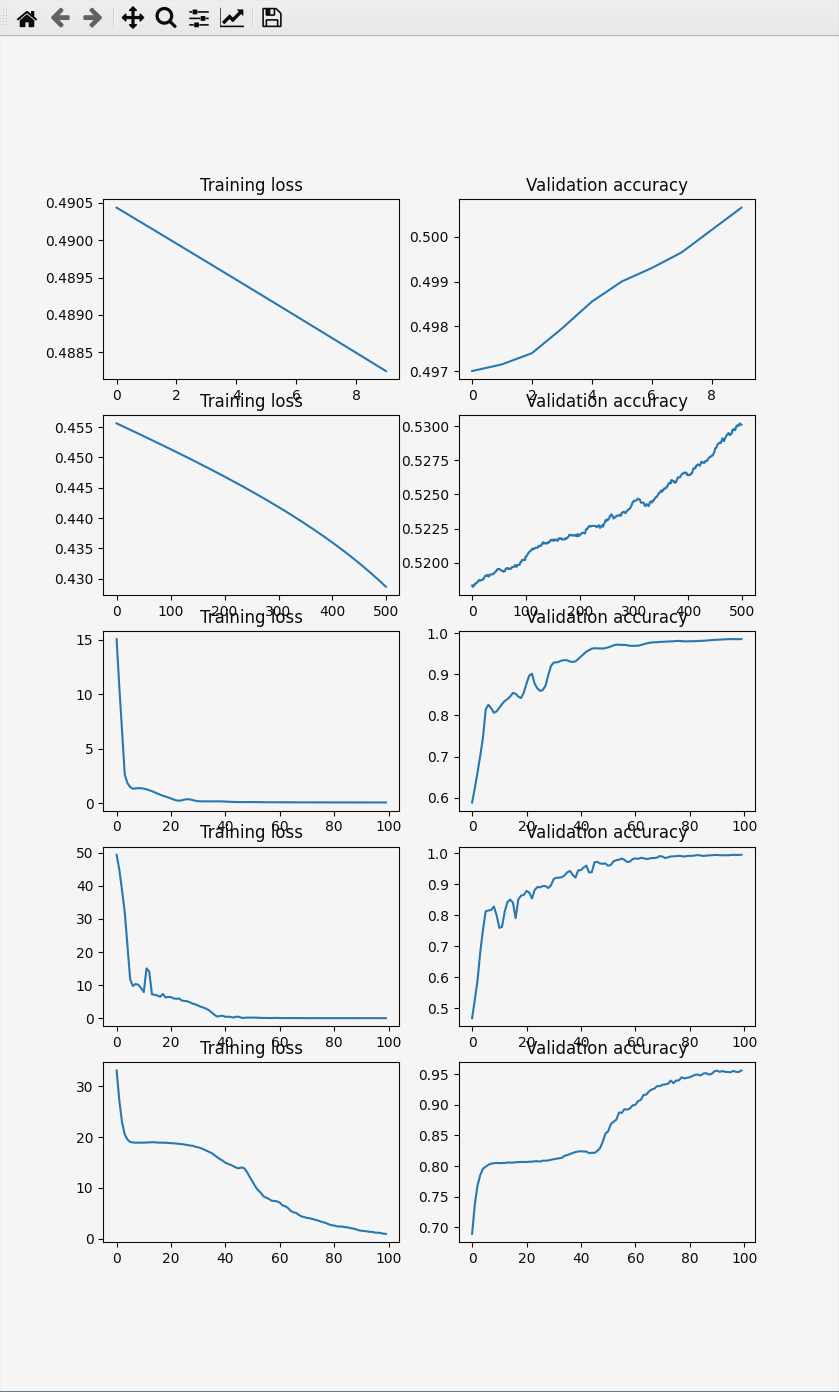
\includegraphics[width=\textwidth]{q5graph}

\end{document}
